\documentclass[12pt]{ximera}
\title{Homework 4: Introduction to Probability}
\begin{document}
\begin{abstract}
Sections 7.3--7.4: converting between odds and probabilities, inclusion-exclusion and
the complement rule for weather events, and a three-set Venn diagram of blood antigen
frequencies.
\end{abstract}
\maketitle

\section*{Sections 7.3--7.4: Probability, Odds, and Venn Diagrams}

\begin{problem}
Suppose the weather report predicts that the odds \emph{against} rain today are $2:3$
and the odds \emph{in favor of} high winds are $3:1$, with $1:1$ odds that both will
occur.

\begin{prompt}
\textbf{(a)} Translate each of the odds given into a probability, as a percentage.

$P(\text{rain})=\answer{60}\%$ \qquad $P(\text{high winds})=\answer{75}\%$ \qquad
$P(\text{both})=\answer{50}\%$

\begin{hint}
Odds of $a:b$ in favor of an event mean probability $\frac{a}{a+b}$. Odds \emph{against}
put the non-occurrences first.
\end{hint}

\begin{feedback}
\begin{itemize}
\item Odds against rain of $2:3$ mean $2$ ``no rain'' for every $3$ ``rain'', so
      $P(\text{rain})=\frac{3}{2+3}=60\%$.
\item Odds in favor of high winds of $3:1$ give $P(\text{winds})=\frac{3}{3+1}=75\%$.
\item Odds of $1:1$ for both give $P(\text{both})=\frac12=50\%$.
\end{itemize}
\end{feedback}
\end{prompt}

\begin{prompt}
\textbf{(b)} Use inclusion-exclusion to find the probability that there will be any rain
or high winds.

$\answer{85}\%$

\begin{feedback}
$P(R\cup W)=P(R)+P(W)-P(R\cap W)=60\%+75\%-50\%=85\%$. Adding $60\%$ and $75\%$ counts
the days with both twice, so one copy of the $50\%$ is subtracted.
\end{feedback}
\end{prompt}

\begin{prompt}
\textbf{(c)} Use the complement rule to find the probability of neither rain nor high
winds.

$\answer{15}\%$

\begin{feedback}
``Neither'' is the complement of ``rain or winds'': $100\%-85\%=15\%$.
\end{feedback}
\end{prompt}

\begin{prompt}
\textbf{(d)} What are the odds in favor of there being \emph{only} high winds? Reduce
your answer.

The odds are $\answer{1}$ to $\answer{3}$.

\begin{feedback}
Only high winds (no rain) has probability $P(W)-P(R\cap W)=75\%-50\%=25\%$, and its
complement is $75\%$. So the odds in favor are $25:75=1:3$.
\end{feedback}
\end{prompt}
\end{problem}

\begin{problem}
On their surface, red blood cells have inherited chemical structures called antigens
that can cause a person's immune system to make antibodies against them. Every human
has a particular combination of antigens on the surface of their blood cells, and
their immune system will create antibodies against any antigens that are not among
their own.

There are many major and minor groups of these antigens, but in particular,
consideration of the presence of A, B, and Rh antigens is necessary to ensure that a
transfusion recipient receives compatible blood.

For example, someone with A antigens but neither B nor Rh antigens (commonly called
``A-negative'' or ``A$-$'' blood type) could donate blood to anyone who has A
antigens (that is, anyone with A$+$, A$-$, AB$+$, or AB$-$ blood type), but could
only receive a transfusion from someone with neither B nor Rh antigens (that is,
anyone with A$-$ or O$-$ blood type, where ``O'' signifies the absence of A or B
antigens).

The following data about blood type frequency was reported by the National Health
Service in 2018. Among blood donors,
\begin{itemize}
    \item $75\%$ have Rh antigens;
    \item $41\%$ have A antigens;
    \item $13\%$ have B antigens;
    \item $32\%$ have Rh and A antigens;
    \item $10\%$ have Rh and B antigens;
    \item $3\%$ have A and B antigens;
    \item $2\%$ have all three of these antigens.
\end{itemize}

\begin{prompt}
\textbf{(a)} Fill in the seven regions of the Venn diagram, as percentages. Work
from the center outward.

\begin{center}
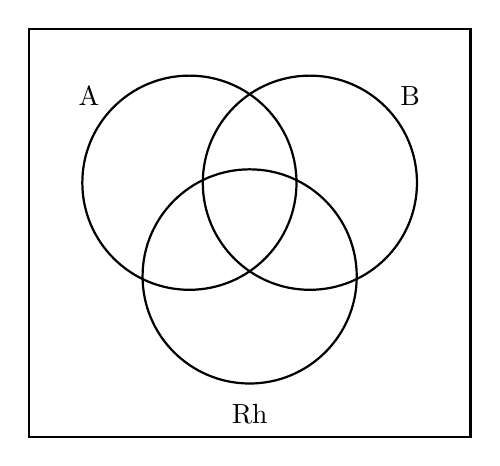
\begin{tikzpicture}[scale=0.85]
  \draw[thick] (-0.9,0.5) circle (1.6) node at (-2.4,1.8) {A};
  \draw[thick] (0.9,0.5) circle (1.6) node at (2.4,1.8) {B};
  \draw[thick] (0,-0.9) circle (1.6) node at (0,-2.95) {Rh};
  \draw[thick] (-3.3,-3.3) rectangle (3.3,2.8);
\end{tikzpicture}
\end{center}

All three antigens (the center): $\answer{2}\%$

\smallskip
A and B but not Rh: $\answer{1}\%$ \qquad
A and Rh but not B: $\answer{30}\%$ \qquad
B and Rh but not A: $\answer{8}\%$

\smallskip
A only: $\answer{8}\%$ \qquad
B only: $\answer{2}\%$ \qquad
Rh only: $\answer{35}\%$

\begin{hint}
Start with the center ($2\%$, given directly) and work outward. Each two-antigen
figure, such as the $3\%$ with A and B, \emph{includes} the people who have all
three --- so subtract the center from it to get the ``exactly these two'' region.
\end{hint}

\begin{feedback}
Start at the center and work out.
\begin{itemize}
\item All three: $2\%$, given.
\item A and B: the $3\%$ includes the $2\%$ with all three, so A and B but not Rh is
      $3-2=1\%$.
\item A and Rh: $32-2=30\%$.
\item B and Rh: $10-2=8\%$.
\item A only: the whole A circle is $41\%$, from which we remove the three regions
      just found that sit inside it: $41-(1+30+2)=8\%$.
\item B only: $13-(1+8+2)=2\%$.
\item Rh only: $75-(30+8+2)=35\%$.
\end{itemize}
\end{feedback}
\end{prompt}

\begin{prompt}
\textbf{(b)} What is the probability that a donor's blood contains none of these
antigens (O$-$)?

$\answer{14}\%$

\begin{hint}
Add up all seven regions inside the circles and subtract from $100\%$.
\end{hint}

\begin{feedback}
The seven regions inside the diagram total
\[ 2+1+30+8+8+2+35 = 86\%, \]
so the region outside all three circles is $100-86=14\%$.
\end{feedback}
\end{prompt}

\begin{prompt}
\textbf{(c)} Per the example above, what is the probability a random donor's blood
type is compatible as a transfusion for someone with A antigens but neither B nor Rh
antigens (A$-$)?

$\answer{22}\%$

\begin{hint}
Re-read the example: an A$-$ recipient can accept blood only from A$-$ or O$-$
donors. Which two regions of your diagram are those?
\end{hint}

\begin{feedback}
An A$-$ recipient can receive blood only from donors with neither B nor Rh antigens,
which is A$-$ blood (the ``A only'' region) or O$-$ blood (the region outside all
three circles). From parts (a) and (b), those are $8\%$ and $14\%$, so
\[ 8\% + 14\% = 22\%. \]
\end{feedback}
\end{prompt}
\end{problem}

\end{document}
